%%%%%%%%%%%%%%%%%%%%%%%%%%%%%%%%%%%%%%%%%%%%%%%%%%%
%% P3: Phenomenology of Particle Physics                         
%%
%% Author:  André Rubbia                   		 
%%
%% Figure 12.7 Measured values of the running coupling constant $\alpha$.
%%
%% This work is licensed under the Creative Commons Attribution 4.0 International License. 
%% To view a copy of this license, visit http://creativecommons.org/licenses/by/4.0/ or 
%% send a letter to Creative Commons, PO Box 1866, Mountain View, CA 94042, USA.
%%
%%%%%%%%%%%%%%%%%%%%%%%%%%%%%%%%%%%%%%%%%%%%%%%%%%%

\documentclass[a4paper,10pt]{article}

\usepackage[T1]{fontenc}
\usepackage[utf8]{inputenc}
\usepackage{lmodern}
\usepackage[labelfont=bf]{caption}
\usepackage{upgreek}

\usepackage{tikz}
\usepackage{pgfplots}
\pgfplotsset{compat=1.17}
\usepgfplotslibrary{ternary}
\usepgfplotslibrary{fillbetween}
\usepgfplotslibrary{external}

\usepackage{braket}

\def\d{\mathrm{d}}

\begin{document}

%%%%%%%%%%%%%%%%% FIGURE %%%%%%%%%%%%%%%%%%%%%%%%%%%%%%%%%%
\begin{figure}[htb]
    \centering
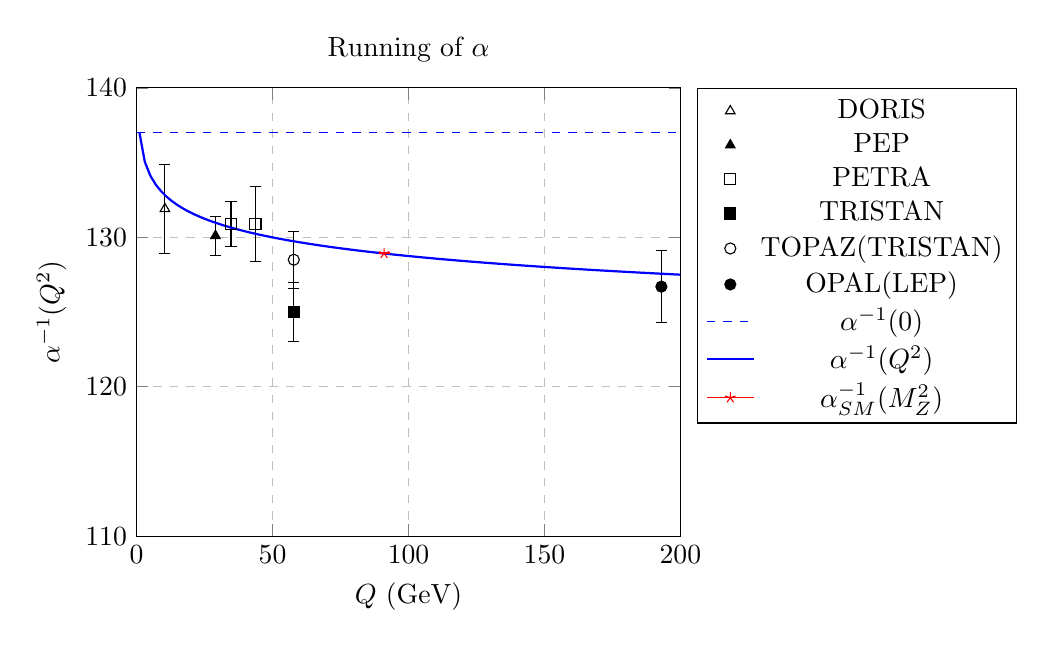
\begin{tikzpicture}[scale=1.]
\begin{axis}[
    width=0.7\textwidth,
    height=0.6\textwidth,
    title={Running of $\alpha$},
    xlabel={$Q$  (GeV)},
    ylabel={$\alpha^{-1}(Q^2)$},
    xmin=0, xmax=200,
    ymin=110, ymax=140,
	legend style={legend pos = outer north east},
    	ymajorgrids=true,
    	xmajorgrids=true,
    grid style=dashed,
]

\addplot[
    only marks,
    mark = triangle,
    error bars/.cd,
    y dir=both, y explicit
    ]
    coordinates {
(10.4,131.9)+-(0,3)
     };

\addplot[
    only marks,
    mark = triangle*,
    error bars/.cd,
    y dir=both, y explicit
    ]
    coordinates {
(29,130.1)+-(0,1.3)
     };

\addplot[
    only marks,
    mark = square,
    error bars/.cd,
    y dir=both, y explicit
    ]
    coordinates {
(34.7,130.9)+-(0,1.5)
(43.7,130.9)+-(0,2.5)
     };

\addplot[
    only marks,
    mark = square*,
    error bars/.cd,
    y dir=both, y explicit
    ]
    coordinates {
(57.8,125.0)+-(0,2.0)
     };

\addplot[
     only marks,
   mark = o,
    error bars/.cd,
    y dir=both, y explicit
    ]
    coordinates {
(57.8,128.5)+-(0,1.9)
     };

\addplot[
     only marks,
    mark = *,
    error bars/.cd,
    y dir=both, y explicit
    ]
    coordinates {
(193,126.7)+-(0,2.4)
     };

\addplot[domain=0:200,
    color=blue,dashed,
    no marks
    ]
  {137.036};

  \addplot[domain=1:200,samples=100,
    color=blue,thick,
    no marks
    ]
  {137.036*(1-1.8*ln(x)/137.036)};

  \addplot[
  color=red,
    mark = star,
    error bars/.cd,
    y dir=both, y explicit
    ]
    coordinates {
(91,128.927)+-(0,0.023)
     };

     \legend{DORIS,
    PEP,
     PETRA,
     TRISTAN,
     TOPAZ(TRISTAN),
     OPAL(LEP),
     $\alpha^{-1}(0)$,
     $\alpha^{-1}(Q^2)$,
     $\alpha_{SM}^{-1}(M_Z^2)$
	}
\end{axis}
\end{tikzpicture}
    \caption{Measured values of the running coupling constant $\alpha$ at the DORIS, PEP, PETRA, TRISTAN, and LEP $e^+e^-$ colliders. The solid line shows the theoretical expectation.}
\end{figure}
%%%%%%%%%%%%%%%%% END FIGURE %%%%%%%%%%%%%%%%%%%%%%%%%%%%%%
%

\end{document}
